\chapter{Bringing It To Fruition}
\label{chap:BringingItToFruition}

At this point in the development of your the\-sis/dis\-ser\-ta\-tion
you have prepared a draft which must now be brought to fruition. This
chapter describes the possible steps for completion and final
acceptance of the final manuscript. These steps are summarized in
Figure \ref{fig:ThesisFlowchart}.
\begin{figure}[tbp]
  \centering
  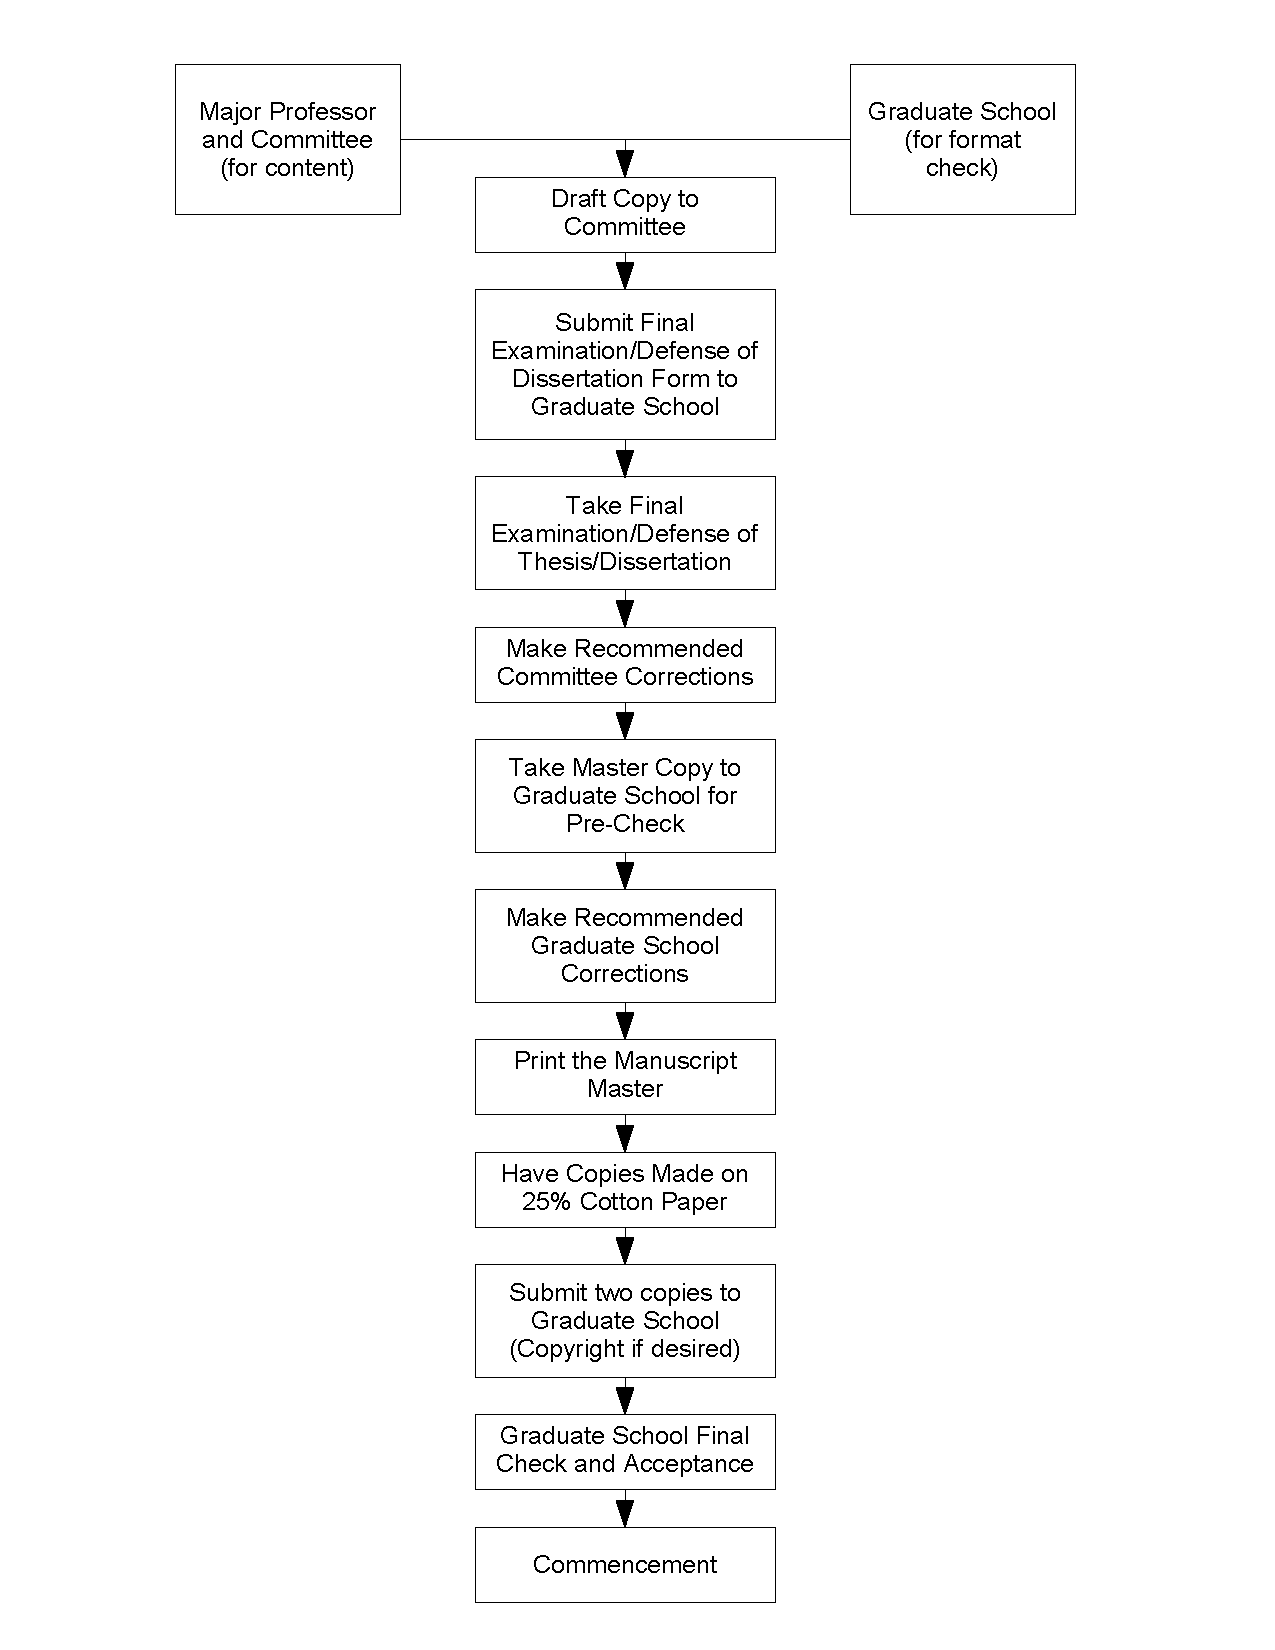
\includegraphics[width=0.9\textwidth]{thesis-manual-content/thesis-flowchart}
  \caption{Sample Flowchart Summarizing Possible Steps to Completion and Acceptance of a The\-sis/Dis\-ser\-ta\-tion}
  \label{fig:ThesisFlowchart}
\end{figure}

\section{Draft Copy to Committee}
\label{sec:DraftCopyToCommittee}

Before you submit a draft copy of your the\-sis/dis\-ser\-ta\-tion to
your committee, it should be checked out by at least your major
professor for content. His/her recommendations should be incorporated
in the draft copy that you submit to your graduate advisory committee.
\textbf{Please note that this review by your major professor is a
  crucial step, and it may need to be repeated several times.}

When your major professor is satisfied with your draft copy, you must
submit a copy to all members of your advisory committee for their
review. At the same time you should set a date, time, and place that
is convenient for all your committee members for the presentation and
final ex\-am\-i\-na\-tion/de\-fense of your
the\-sis/dis\-ser\-ta\-tion. This date should be no sooner than one
week after you submit your draft copy to them.

\subsection{Final Examination/Defense of Thesis/Dissertation}
\label{sec:FinalExaminationDefenseOfThesisDissertation}

The format of your presentation and final examination and/or defense
of your the\-sis/dis\-ser\-ta\-tion (which in some departments
requires more than one session) is set by the policy of your
department or college.  Although its length may vary with whether it
is for a thesis or dissertation, there is typically a formal oral
presentation of your research to your advisory committee and any
guests whom you or your committee members might have invited. A period
for questions normally follows. The intention of this process is to
verify your understanding of your contribution to the body of
knowledge in your research area and your general field of study.

\subsection{Committee Revisions}
\label{sec:CommitteeRevisions}

Recommendations for changes and/or additions are a natural
by\-prod\-uct of this review of your the\-sis/dis\-ser\-ta\-tion by
your entire committee and your defense of it. These should be
critically reviewed with both your major professor and the individual
committee members who made the recommendation, and incorporated as
appropriate.

\subsection{Graduate School Pre-check}
\label{sec:GraduateSchoolPrecheck}

At this point your manuscript is ready for a pre-check by the Graduate
School prior to its final approval by your advisory committee and
submission to the printer for reproduction. This pre-check will pick
up any format problems that must be corrected before the
the\-sis/dis\-ser\-ta\-tion is printed. The Graduate School must
receive, by the date published in the Bulletin, one preliminary copy
of the the\-sis/dis\-ser\-ta\-tion for pre-check. Failure to submit
the preliminary copy by the deadline will result in your removal from
the commencement list.

\section{Graduate School Revisions}
\label{sec:GraduateSchoolRevisions}

You must now make the revisions recommended by the Graduate School. If
there is any doubt about a revision, check with the Graduate School
again. This is also the appropriate time to take a copy of your
manuscript to each of your advisory committee members to obtain their
final approval of your the\-sis/dis\-ser\-ta\-tion, as reflected by
their signature on your Certificate of Approval of
The\-sis/Dis\-ser\-ta\-tion.

\section{Printing the Manuscript Master}
\label{sec:PrintingTheManuscriptMaster}

\textbf{Under no circumstances should you generate the two final
  copies from a printer.} You must photocopy them from the manuscript
master onto 25 percent cotton content, 20 pound paper. The surface of
cotton paper is such that ink from nonimpact printers does not always
adhere permanently. The general premise of most photocopying is a
combination of heat and pressure which produces a stronger permanent
bond of the ink or toner with the paper. Although some printers
function in much the same way, neither the heat or pressure is
sufficient to assure a permanent bond to 25 percent cotton paper. This
is a potential problem of all nonimpact printers. The problem has been
noted on various brands of cotton paper and with a variety of
printers. In some cases there has been flaking on random pages or
smearing of copy from pages rubbing against each other.

The printer quality should be sufficient to produce a smooth,
high-contrast copy. The poor quality of low-density dot matrix print
is not acceptable.

\section{Copying}
\label{sec:Copying}

ou will find area copy shops that are familiar with the University's
requirements concerning paper and copy quality. The cost of having
copies made by local shops is reasonable, and you will save little
money by buying your paper and doing your own copying. Professional
shops are responsible for equipment malfunctions and should maintain a
supply of 25 percent cotton paper.

All brands of 20 pound, 25 percent cotton paper are acceptable, but
all pages, including the approval sheets and any outsize pages
(11$\times$17 inches), must be on the same brand. If you are an
out-of-town student, you may wish to investigate copy shops in your
location for comparison with those in this area. Often local shops
will make arrangements to accept the master copy by mail, make the
copies, and deliver them to the Graduate School for a fee.

\section{Submission to Graduate School}
\label{sec:SubmissionToGraduateSchool}

\subsection{Official Copies}
\label{sec:OfficialCopies}

The Graduate School must receive, by the date published in the
Bulletin, two official copies of the the\-sis/dis\-ser\-ta\-tion,
including the Certificate of Approval of The\-sis/Dis\-ser\-ta\-tion
with original signatures, on 20 pound 25 percent cotton paper in an
8.5$\times$11 inch file folder. These two official copies will be
hard-bound and placed in the Tennessee Technological University
Library under arrangements made by the Graduate School. Doctoral
students must provide one additional copy for microfilming by
University Microfilms International of Ann Arbor, Michigan. This
constitutes publication and makes the dissertation available to the
public. Your department may require additional copies of your
the\-sis/dis\-ser\-ta\-tion.

\subsection{Additional Copies and Binding}
\label{sec:AdditionalCopiesAndBinding}

You are also responsible for the reproduction of all other copies of
the the\-sis/dis\-ser\-ta\-tion. Hard binding of these copies may be
arranged through the Graduate School. Your major professor can help
determine who expects to receive copies and how they should be bound.

\subsection{Copyright}
\label{sec:AssigningCopyright}

If the research work for your thesis or dissertation was supported in
part by a contract or grant, you should check with your major advisor
relative to any restrictions that might apply to copyrighting the
material. After consultation with the chairperson of your advisory
committee, you should decide whether or not to copyright the thesis to
discourage unauthorized copying. If you decide to copyright, you must
insert an extra page after the title page of each volume. Assign this
page the number ii, but do not type the number on the page. Type and
center the following information on the copyright page:
\begin{center}
  \begin{tabular}[h]{|c|} \hline
    Copyright \copyright $\underbar{\quad\quad\quad\quad\quad}$, 20 (year) \\
    All rights reserved \\ \hline
  \end{tabular}
\end{center}

Registration of your the\-sis/dis\-ser\-ta\-tion document with the
U.S.  Copyright Office is optional. Once the copyright notice is
placed in the document, it is fully protected by the Copyright Law;
however, registration is a prerequisite to certain remedies for
infringement.

In view of the University's Policy on Patents and Copyrights, with
regard to the\-sis/dis\-ser\-ta\-tion support, you should consult the
chairperson of your advisory committee before the copyright notice is
placed in the document. A copy of the University Policy is available
in the Office of Research.

\section{Graduate School Final Check and Acceptance}
\label{sec:GraduateSchoolFinalCheckAndAcceptance}

After you have submitted the final copies to the Graduate School, that
office will review your the\-sis/dis\-ser\-ta\-tion again for
corrections made on any previous errors and will count the pages. When
this review has been successfully completed, your
the\-sis/dis\-ser\-ta\-tion will be approved.

\section{Commencement}
\label{sec:Commencement}

Commencement is a fitting culmination of your effort to obtain a
graduate degree. Whatever the degree to be conferred, it marks an
appropriate beginning.

%%% Local Variables: 
%%% mode: latex
%%% TeX-master: "thesis"
%%% End: 
